\documentclass{article}

% if you need to pass options to natbib, use, e.g.:
%     \PassOptionsToPackage{numbers, compress}{natbib}
% before loading neurips_2026
\PassOptionsToPackage{numbers,compress}{natbib}

% The authors should use one of these tracks.
% Before accepting by the NeurIPS conference, select one of the options below.
% 0. "default" for submission
\usepackage{neurips_2026}

% the "default" option is equal to the "main" option, which is used for the Main Track with double-blind reviewing.
% 1. "main" option is used for the Main Track
%  \usepackage[main]{neurips_2026}
% 2. "position" option is used for the Position Paper Track
%  \usepackage[position]{neurips_2026}
% 3. "eandd" option is used for the Evaluations & Datasets Track
 % \usepackage[eandd]{neurips_2026}
% 4. "creativeai" option is used for the Creative AI Track
%  \usepackage[creativeai]{neurips_2026}
% 5. "sglblindworkshop" option is used for the Workshop with single-blind reviewing
 % \usepackage[sglblindworkshop]{neurips_2026}
% 6. "dblblindworkshop" option is used for the Workshop with double-blind reviewing
%  \usepackage[dblblindworkshop]{neurips_2026}

% After being accepted, the authors should add "final" behind the track to compile a camera-ready version.
% 1. Main Track
 % \usepackage[main, final]{neurips_2026}
% 2. Position Paper Track
%  \usepackage[position, final]{neurips_2026}
% 3. Evaluations & Datasets Track
 % \usepackage[eandd, final]{neurips_2026}
% 4. Creative AI Track
%  \usepackage[creativeai, final]{neurips_2026}
% 5. Workshop with single-blind reviewing
%  \usepackage[sglblindworkshop, final]{neurips_2026}
% 6. Workshop with double-blind reviewing
%  \usepackage[dblblindworkshop, final]{neurips_2026}
% Note. For the workshop paper template, both \title{} and \workshoptitle{} are required, with the former indicating the paper title shown in the title and the latter indicating the workshop title displayed in the footnote.
% For workshops (5., 6.), the authors should add the name of the workshop, "\workshoptitle" command is used to set the workshop title.
% \workshoptitle{WORKSHOP TITLE}

% "preprint" option is used for arXiv or other preprint submissions
 % \usepackage[preprint]{neurips_2026}

% to avoid loading the natbib package, add option nonatbib:
%    \usepackage[nonatbib]{neurips_2026}

\usepackage[utf8]{inputenc} % allow utf-8 input
\usepackage[T1]{fontenc}    % use 8-bit T1 fonts
\usepackage{hyperref}       % hyperlinks
\usepackage{url}            % simple URL typesetting
\usepackage{booktabs}       % professional-quality tables
\usepackage{amsfonts}       % blackboard math symbols
\usepackage{amsmath}        % mathematical text and aligned equations
\usepackage{nicefrac}       % compact symbols for 1/2, etc.
\usepackage{microtype}      % microtypography
\usepackage{xcolor}         % colors
\usepackage{graphicx}       % figures
% Note. For the workshop paper template, both \title{} and \workshoptitle{} are required, with the former indicating the paper title shown in the title and the latter indicating the workshop title displayed in the footnote.
\title{When Delay Meets Distribution Shift:\\ Evaluating Asynchronous Vision-Language-Action Policies}


% The \author macro works with any number of authors. There are two commands
% used to separate the names and addresses of multiple authors: \And and \AND.
%
% Using \And between authors leaves it to LaTeX to determine where to break the
% lines. Using \AND forces a line break at that point. So, if LaTeX puts 3 of 4
% authors names on the first line, and the last on the second line, try using
% \AND instead of \And before the third author name.


\author{%
  Anonymous Authors \\
  % examples of more authors
  % \And
  % Coauthor \\
  % Affiliation \\
  % Address \\
  % \texttt{email} \\
  % \AND
  % Coauthor \\
  % Affiliation \\
  % Address \\
  % \texttt{email} \\
  % \And
  % Coauthor \\
  % Affiliation \\
  % Address \\
  % \texttt{email} \\
  % \And
  % Coauthor \\
  % Affiliation \\
  % Address \\
  % \texttt{email} \\
}


\begin{document}
\maketitle

\begin{abstract}
Asynchronous execution allows continuous movement in a robot while its policy computes the next action chunk in the background. However, this form of execution comes with two risks: the actions remaining in the queue could be predicted from a stale observation, and the queue may be exhausted before the inference finishes. This paper examines whether distribution shifts make inference delay more harmful. We use a fixed LIBERO-fine-tuned $\pi_{0.5}$ checkpoint and compare matched LIBERO and LIBERO-Plus conditions using a discrete-event executor. For each request, it combines measured inference latency with an added logical delay. We select $+200\,\mathrm{ms}$ using in-distribution (ID) trials only, then apply it to both ID and out-of-distribution (OOD) conditions. Across the pooled Naive Async and Real-Time Chunking (RTC) screen, we do not observe a larger delay-related success drop under OOD than under ID. Action coverage shows a clearer difference. In ID-only RTC tests at $+200\,\mathrm{ms}$, 10 configured actions give $6/15$ successful episodes, compared with $14/15$ at each of 20, 25, and 30 actions. Our 64-seed held-out follow-up finds mixed, horizon-dependent local interactions. The previously negative long-stove/object-layout effect changes sign by $h=30$, while most paired-bootstrap intervals include zero. We therefore suggest checking action coverage against the tested delay before attributing failures to distribution shift. Our complete implementation and benchmark suite are publicly available at: https://anonymous.4open.science/r/vla-latency-benchmark-23CB/README.md.



\end{abstract}


\section{Introduction}

    Most modern Vision-language-Action policies predict temporally extended action chunks rather than a single action at each control step which not only enables coherent behavior but also reduces the frequency of policy replanning \cite{1}\cite{2}. Generating a new chunk isn't instantaneous and may span multiple controller steps. In such cases, synchronous execution may pause control while asynchronous execution allows the robot to continue acting \cite{3}. While  this overlap aims to preserve control throughput, it results in actions being executed (during inference) on an increasingly stale observation. Consequently, robustness of asynchronous operations is not only a result of policy quality, but also whether there are still sufficient numbers of actions left in the current block to last until the next prediction comes through.

\begin{figure}[h]
    \centering
    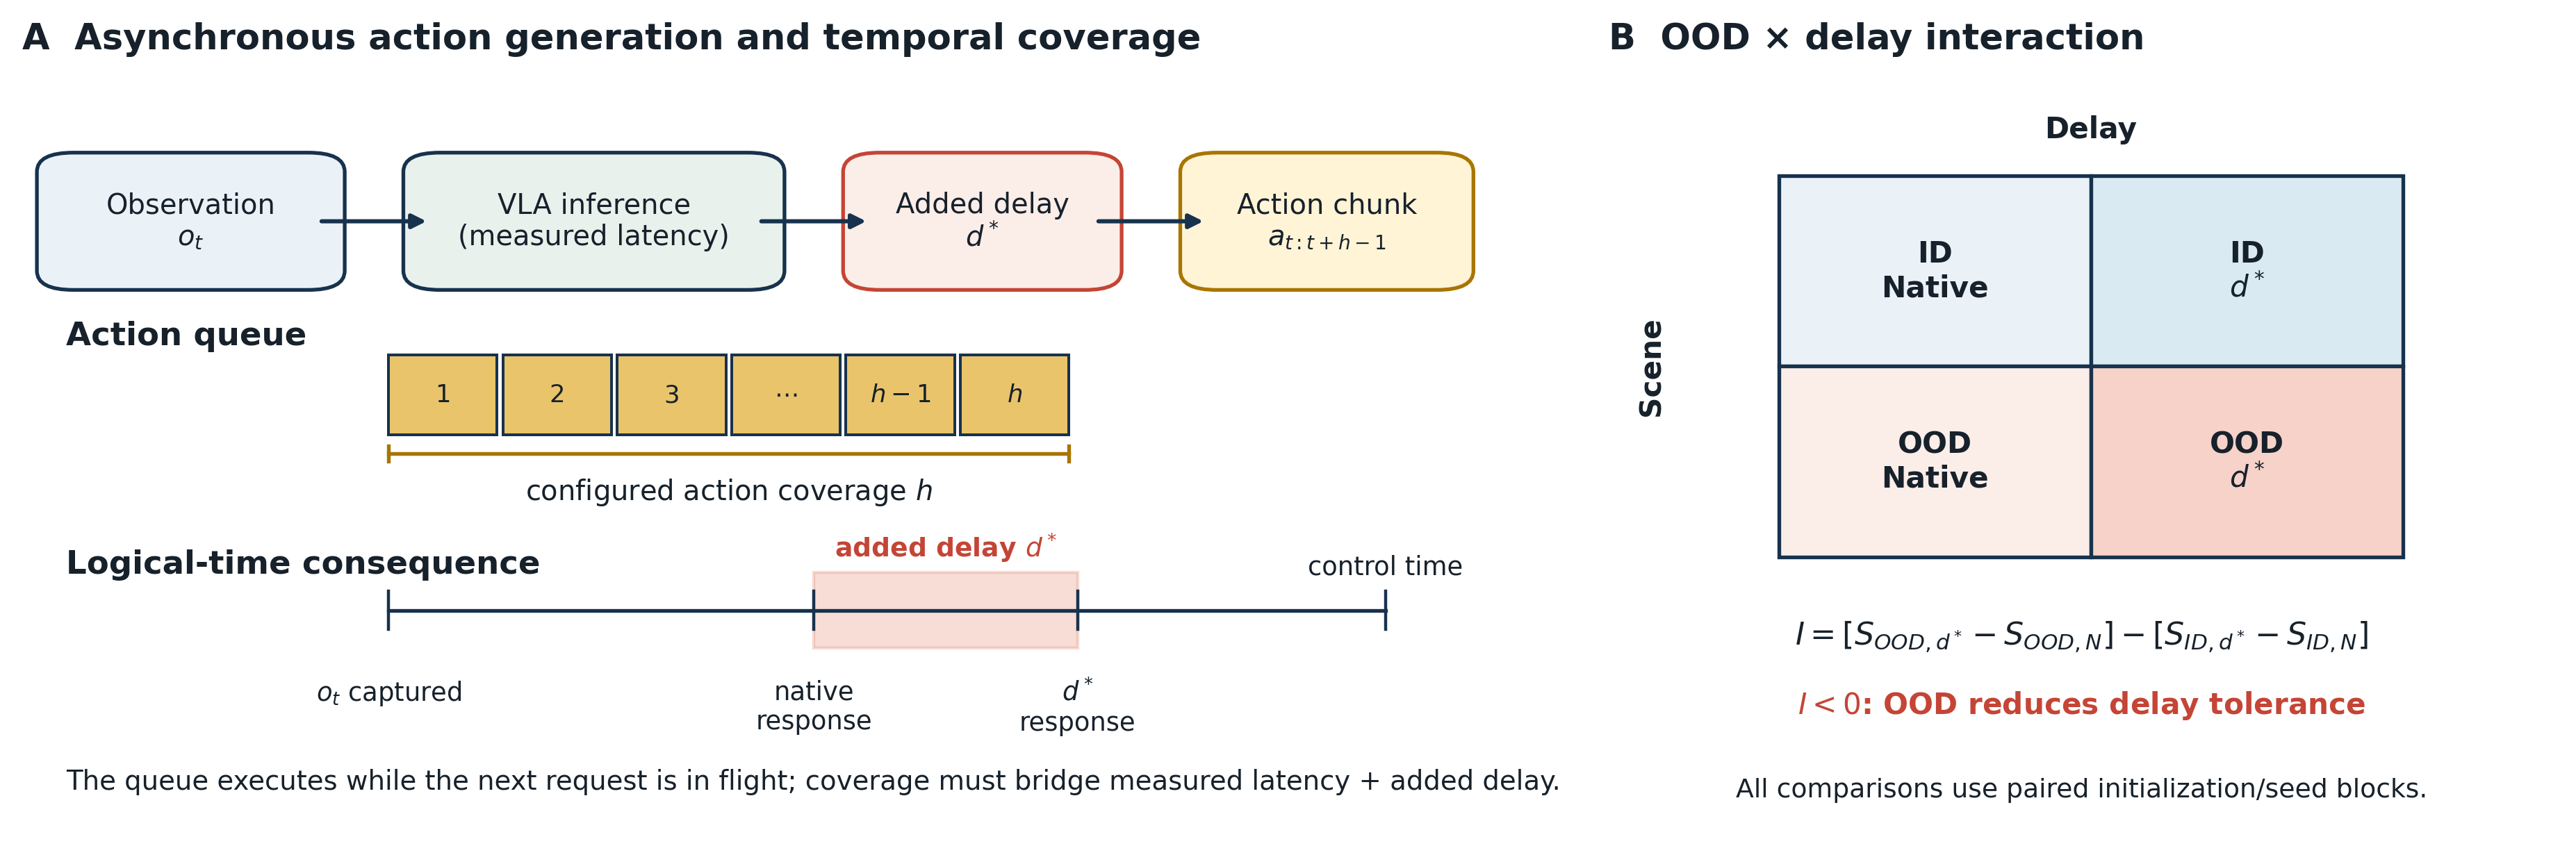
\includegraphics[width=\textwidth]{figure1_experimental_concept.png}
    \caption{Illustration of the control interruption caused by blocking action-chunk inference and the overlapping execution used by streaming asynchronous control.}
    \label{fig:inference_flow}
\end{figure}

    Current research has examined various aspects of this problem. Real-Time Chunking(RTC) and further studies examine the behavior of asynchronous execution methods under varying inference delays and action-chunk lengths. These studies show that their relative performance depends on delay regime, underlying policy, and evaluation benchmark  \cite{3}\cite{4}. Separately, LIBERO-Plus assess VLA policies under controlled variations in object layout, camera viewpoint, robot initial state, lighting, background texture, language instructions, and sensor noise \cite{5}. However, they fail to isolate the effects of inference delay on observation staleness while providing the required coverage of actions. Per these benchmarks, static out-of-distribution(OOD) success measures sensitivity to environmental change, while delayed ID execution measures sensitivity to stale control. Whether an environmental shift changes the additional penalty caused by asynchronous delay remains under-characterized.

We study this interaction using a fixed implementation of $\pi_{0.5}$ checkpoint on three selected base tasks from LIBERO \cite{6}, pairing their standard ID instances with exact pre-generated OOD task variants from LIBERO-Plus \cite{5}. For each policy request, our executor uses the measured inference time, adds the chosen delay on the logical control clock, and records which observation and action chunk each executed action came from. We choose $+200\,\mathrm{ms}$ using ID runs only and compare Naive Async and RTC in a broad ID/OOD screen. Next, we test RTC with different numbers of configured actions. Selected OOD conditions are rerun with 64 rollout seeds per cell. We find that across the broad screen, the added delay does not produce a larger pooled success drop under OOD than under ID. However, performance does seem to be more clearly affected by the number of available actions. The high-power held-out results are mixed and horizon-dependent rather than a universal OOD amplification pattern. These findings suggest that delay should be calibrated against available action coverage before failures are attributed to distribution shift.


\section{Related Work}

Temporal action forecasting has become common in robot learning tasks: ACT uses action sequences via transformers, Diffusion Policy combines diffusion-based trajectory prediction with receding-horizon control, and the $\pi_0$/$\pi_0._5$ family uses action chunks through flow matching \cite{1} \cite{8} \cite{9} \cite{10}. Action chunks improve temporal consistency and amortize inference costs, but executing several actions before re-planning means new observations affect control less frequently \cite{3}\cite{11}. Recent works therefore consider the execution horizon: AutoHorizon estimates a horizon for each chunk, while DEHP learns an additional horizon-selection module \cite{12}\cite{13}. RTC addresses a related problem, inference latency, by reconciling a new chunk with actions already committed \cite{3}.

The high inference latency of VLA creates two undesirable modes: synchronous control pauses while waiting, whereas asynchronous control continues with actions derived from stale observations \cite{3} \cite{14} \cite{11} \cite{15}. Existing approaches address this mismatch at different pipeline stages. Inference-time RTC preserves the committed action prefix and inpaints the remainder of the incoming chunk, whereas training-time RTC simulates delay during training \cite{3} \cite{16}. VLASH and FutureRTC estimate the state or observation expected at execution time, while A2C2 and Action ControlNet introduce lightweight delay-aware corrections \cite{11} \cite{14} \cite{15} \cite{17}. An evaluation of IT-RTC, TT-RTC, VLASH, and A2C2 across Kinetix and LIBERO further shows that their relative performance varies with delay, chunk length, base policy, and benchmark \cite{18}. These studies mainly focus on the development or comparison of mechanisms for avoiding delayed execution. We use Naive Async only exploratorily and keep RTC fixed for confirmatory analysis, while recording observation and chunk provenance for each action. This will allow us to analyze temporal provenance along with the measured latency.

Evaluation of robot policies is increasingly moving beyond their effectiveness in nominal scenarios to determine how well they perform in dealing with visual, semantic, and behavioral variations \cite{6} \cite{19} \cite{20}. LIBERO offers 130 manipulation tasks in  four suites based on language, whereas LIBERO-Plus enhances the above framework with perturbations across seven dimensions: object layout, camera viewpoint, robot initial state, language instruction, lighting, background texture, and sensor noise \cite{6} \cite{5}. Related studies have found VLA to be highly susceptible to view-point changes, visual, instructional, and multimodal perturbations, and recent research seeks to recover performance through targeted visual adaptation or robustness training \cite{5} \cite{21} \cite{22}. These studies focus on measuring success with perturbation or building adaptation methods, while asynchronous-control experiments mainly focus on the manipulation of inference delay in a scenario where there is no matched comparison between ID and OOD environments  \cite{3} \cite{4}. We connect these two lines of work by measuring the effect of the same added delay under matched ID and OOD conditions.

\section{Method}
\label{gen_inst}
\subsection{Asynchronous VLA Execution}

Although \(\pi_{0.5}\) generates a 50-action chunk, usually only a part of the generated action chunk is added to the action queue to be executed by the robot. We refer to the number of actions made available to the robot for execution as the execution horizon \(h\). Action coverage refers to the amount of time the robot can continue executing these generated actions before it runs out of actions to perform. For example, if the execution horizon is 25 actions and the robot is moving at a 20 Hz control frequency, the action coverage becomes
\[
25 \times 50\,\mathrm{ms} = 1250\,\mathrm{ms}.
\]
The VLA takes some time to process a given observation and compute the next action chunk. This time is referred to as request latency. During asynchronous execution, while a new policy request is being computed, the robot can continue executing actions that are already present in its current action queue. Usually, it's ideal that the response latency be less than the action coverage so that before the queue of actions gets empty, the robot gets fresh new actions queue to execute.

If the robot exhausts all currently available policy-generated actions before the new policy response becomes available, we say that a queue underrun occurs. In such a case, the robot's fallback action is called a hold action. A hold action is a default control action that is executed until a new policy-generated action becomes available.

\subsection{Execution Strategies}

\subsubsection{Naive Asynchronous Execution}

In the Naive Asynchronous execution method, the robot keeps executing the actions already present in its action queue while waiting for the policy to return the next chunk of actions. Let \(a\) be the total number of actions that the policy generates for a given observation, and let \(h\) be the number of actions from that chunk that are added to the robot's action queue for execution. Let $r$ denote the request threshold, defined as the number of remaining queued actions at which the controller sends the latest observation to the policy to generate a new set of $a$ actions. While the new policy request is being processed, the robot continues executing the actions that remain in the current queue.

If the policy returns the new action chunk before all the remaining actions in the queue are executed, the remaining old actions are discarded and the first \(h\) actions from the new chunk are added to the queue. If the policy does not return before all the actions in the queue are executed, a queue underrun occurs and the robot performs a hold action until the next policy-generated action becomes available.

\subsubsection{Real-Time Chunking}
RTC is designed to reduce the temporal mismatch between the newly generated actions and the robot state at the time those actions are executed. When the request threshold is reached, RTC takes into account the remaining actions in the robot's queue and the expected inference delay while generating the next \(a\) actions. For example, if there are 20 remaining actions in the queue and the expected inference delay is 5 control steps, RTC assumes that the first 5 of those actions will already have been executed by the time the new policy response becomes available. These actions are treated as already committed, while the remaining overlapping actions are used to guide the beginning of the newly generated action chunk. While Naive Asynchronous execution generates the new chunk independently of the remaining actions in the old queue and replaces the old remainder when the response arrives, RTC uses the overlap between the old and new chunks to make the transition between them more temporally consistent, reducing abrupt mismatches between already committed actions and newly generated actions.

\subsection{Logical Latency Modeling}
In this paper, we model each response on the logical control clock. For measured policy request latency and injected delay,
$L_{\mathrm{total}} = L_{\mathrm{native}} + L_{\mathrm{added}}$. At 20 Hz, each control step, \(T_{\mathrm{c}}\), is 50 ms. We compute \textit{k}, which is the total latency in control steps, by dividing the total latency by 50 ms and rounding up. If a request is sent at control step \(t_r\) then the new action chunk is only made available after those delay steps have passed.
Until the new chunk of actions are generated, the robot keeps executing the actions that are already present in the queue. The robot executes the hold action if the queue becomes empty before the new response is available.

\subsection{Distribution Shifts}
The $\pi_0._5$ policy is trained on a diverse mixture of robot and non-robot data, including cross-embodiment robot demonstrations and multimodal web data. In our experiments, we define the original LIBERO task configuration as the in-distribution (ID) setting. The out-of-distribution (OOD) setting consists of the same LIBERO tasks with controlled perturbations applied to the environment or task input. For the OOD settings, the final task goal remains the same as in the corresponding ID task, while only the selected perturbation is changed. We use the OOD perturbations to study if adding inference delay has a larger effect when the policy is already operating under a distribution shift. To study this interaction, we compare task performance under ID and OOD conditions at both native and high-delay settings.

\subsection{Evaluation Metrics}
\subsubsection{Task Success}
We report binary task success for each episode and compute success rate as the number of successful episodes divided by the total number of valid episodes.
\subsubsection{Queue Underruns}
A queue underrun occurs when the controller has no policy-generated action available at a control step and must execute the hold action. We report the number or rate of underrun control steps for each condition.
\subsubsection{OOD × Delay Interaction}
To measure whether distribution shift amplifies sensitivity to inference delay, we compute

\[
I =
\left(
S_{\mathrm{OOD,high}}
-
S_{\mathrm{OOD,native}}
\right)
-
\left(
S_{\mathrm{ID,high}}
-
S_{\mathrm{ID,native}}
\right)
\]

Negative values indicate that delay causes a larger performance drop under OOD than under ID, while values near zero indicate little additional interaction between distribution shift and delay.

\section{Experiments}
\label{headings}

\subsection{Compute and Benchmark Setup}
All experiments use one NVIDIA A100 40 GB GPU per worker and use the LeRobot \texttt{lerobot/pi05\_libero\_finetuned} checkpoint for all experiments. We
run one task/episode at a time with no request batching, data
parallelism, or model parallelism. Each worker is pinned to an idle
GPU; GPU/driver identity is recorded and CUDA is synchronized
around measured inference. Native latency is measured independently for each request and combined with injected logical delay.

\subsubsection{Setting the Delay Condition}

We calibrate the added inference delay using only in-distribution LIBERO tasks. We then freeze a single non-saturating high-delay level and use that same delay for every LIBERO-Plus perturbation, task group, and asynchronous execution method.
 The delay intervals were of 0, 100, 200, 300, 400 ms (180 episodes).
The purpose of this was to prevent high-delay setting from being chosen after seeing which OOD conditions produce the strongest results.

\subsubsection{Selecting a Non-Saturating Delay Level}

For each candidate added delay $d \in \{100, 200, 300, 400\}$ ms, evaluated
against the native-latency baseline ($d = 0$), we first restrict to
\emph{viable} ID cells: for each of the six task$\times$method combinations
(3 tasks $\times$ 2 execution methods), a cell is viable for calibration if
\begin{equation}
    S_{\text{native}} \geq 3/6.
\end{equation}
Cells falling below this threshold are retained in all reported tables but
are excluded from determining $d^*$, since they are already near floor under
native latency.

Among the viable cells, we freeze the smallest candidate $d$ satisfying both
\begin{align}
    S_{\text{native}} - S_d &\geq 0.20, \\
    S_d &\geq 0.25,
\end{align}
where $S_{\text{native}}$ and $S_d$ denote pooled success rate under native
and added-delay-$d$ conditions, respectively, pooled over the viable cells
and all six seeds. The first condition ensures the delay manipulation
produces a visible effect (at least a 20 percentage-point drop in success);
the second ensures the resulting condition is not saturated (at least 25\%
success remains at $d$).
Using this predefined criterion, we select $d^*$ = 200 ms as the non-saturating high-delay condition.

\subsection{Testing for Broad OOD Amplification of Delay}

We take 3 tasks and run them across 7 perturbation families, 2 delay conditions and 2 execution methods (naive async, RTC) for 5 seeds each along with 60 shared ID control episodes which result in 480 total analysis episodes. For this experiment, the execution horizon is $h=25$ and the request threshold is $r=25$ actions. For every condition, we compute the OOD delay interaction \textit{I} defined in Section 3.5.

\subsection{Isolating The Role Of Action Horizon}
We vary the execution horizon h to change the amount of temporal action
coverage available while the next request is in flight. Under RTC, we
evaluate h in {10, 15, 20, 25, 30, 35} with Native, +100, +200, and +300 ms delay. A Native baseline is measured at every horizon.

\subsection{Localizing OOD--Delay Effect Across Tasks and Scenes}

We perform fresh-rollout replication with 64 rollout seeds per cell to determine whether the strongest candidate task--perturbation interactions persist across new seeds and execution horizons. We evaluate \texttt{long\_stove\_moka} $\times$ \texttt{object\_layout}, \texttt{goal\_drawer} $\times$ \texttt{robot\_initial\_state}, and \texttt{goal\_drawer} $\times$ \texttt{light\_conditions} under RTC at $h \in \{20,25,30\}$. We additionally include a post-hoc sensor-noise replication and targeted object-layout comparisons on \texttt{spatial\_transport} and \texttt{goal\_drawer}.

We then test object-layout
transfer to (\texttt{spatial\_transport}) and (\texttt{goal\_drawer}) , followed by three
additional \texttt{long\_stove\_moka} layouts and three variants of a second multi-stage task at \textit{h} = 25

\subsection{Initialization Diversity Audit}
We reset each selected OOD variant across requested initialization indices 0--7 and compare environment-state fingerprints to determine whether the indices expose distinct reset states.



\section{Results}

\subsection{Temporal Action Coverage Determines Delay Robustness}

We first study how the execution horizon \(h\) affects robustness to inference delay under RTC. Figure~\ref{fig:operating_envelope} shows pooled task success as \(h\) is varied from 10 to 35 actions. At short horizons, increasing delay causes a sharp degradation in performance. For \(h=10\), success decreases from 93.3\% under Native latency to 40.0\% at +200 ms and 33.3\% at +300 ms. In contrast, larger horizons remain substantially more stable. At \(h=20\), success remains 93.3\% through +200 ms and decreases only to 86.7\% at +300 ms, while \(h=25\) achieves 100\% success under Native latency and 93.3\% at +200 ms.

The queue behavior provides a direct explanation for the failure at short horizons. At \(h=10\), the controller experiences 1,385 queue-underrun control steps at +200 ms and 1,765 at +300 ms. In comparison, no underruns occur at \(h=20\) under +200 ms, and no underruns occur for \(h\geq25\) over the tested delay range. Thus, the sharp degradation at short horizons coincides with the controller exhausting its available policy-generated actions before the next response becomes available. The main OOD operating point of \(h=25\) and +200 ms lies within a comparatively stable region rather than directly at this queue-exhaustion boundary.

\subsection{Distribution Shift Does Not Broadly Amplify Delay Sensitivity}

We next test whether inference delay becomes more damaging when the policy is evaluated under distribution shift. Across the 480-episode broad OOD screen, pooled ID success decreases from 60.0\% under Native latency to 56.7\% at +200 ms, while OOD success decreases from 60.0\% to 58.1\%. Table~\ref{tab:broad_ood} summarizes these results for Naive Async, RTC, and the pooled evaluation. This corresponds to an OOD--delay interaction of approximately \(+0.014\). Since negative values indicate a larger delay-induced degradation under OOD than under ID, the pooled result does not support the hypothesis that distribution shift generally amplifies delay sensitivity.

\begin{table}[t]
\centering
\small
\caption{Success under the ID/OOD \(\times\) Native/+200 ms factorial evaluation.}
\label{tab:broad_ood}
\begin{tabular}{l|cc|c}
\hline
Method & ID Native / +200 & OOD Native / +200 & \(I\) \\
\hline
Naive Async & 33.3\% / 26.7\% & 37.1\% / 33.3\% & \(+0.028\) \\
RTC & 86.7\% / 86.7\% & 82.9\% / 82.9\% & \(0.000\) \\
\hline
Pooled & 60.0\% / 56.7\% & 60.0\% / 58.1\% & \(+0.014\) \\
\hline
\end{tabular}
\end{table}

\begin{figure}[t]
    \centering
    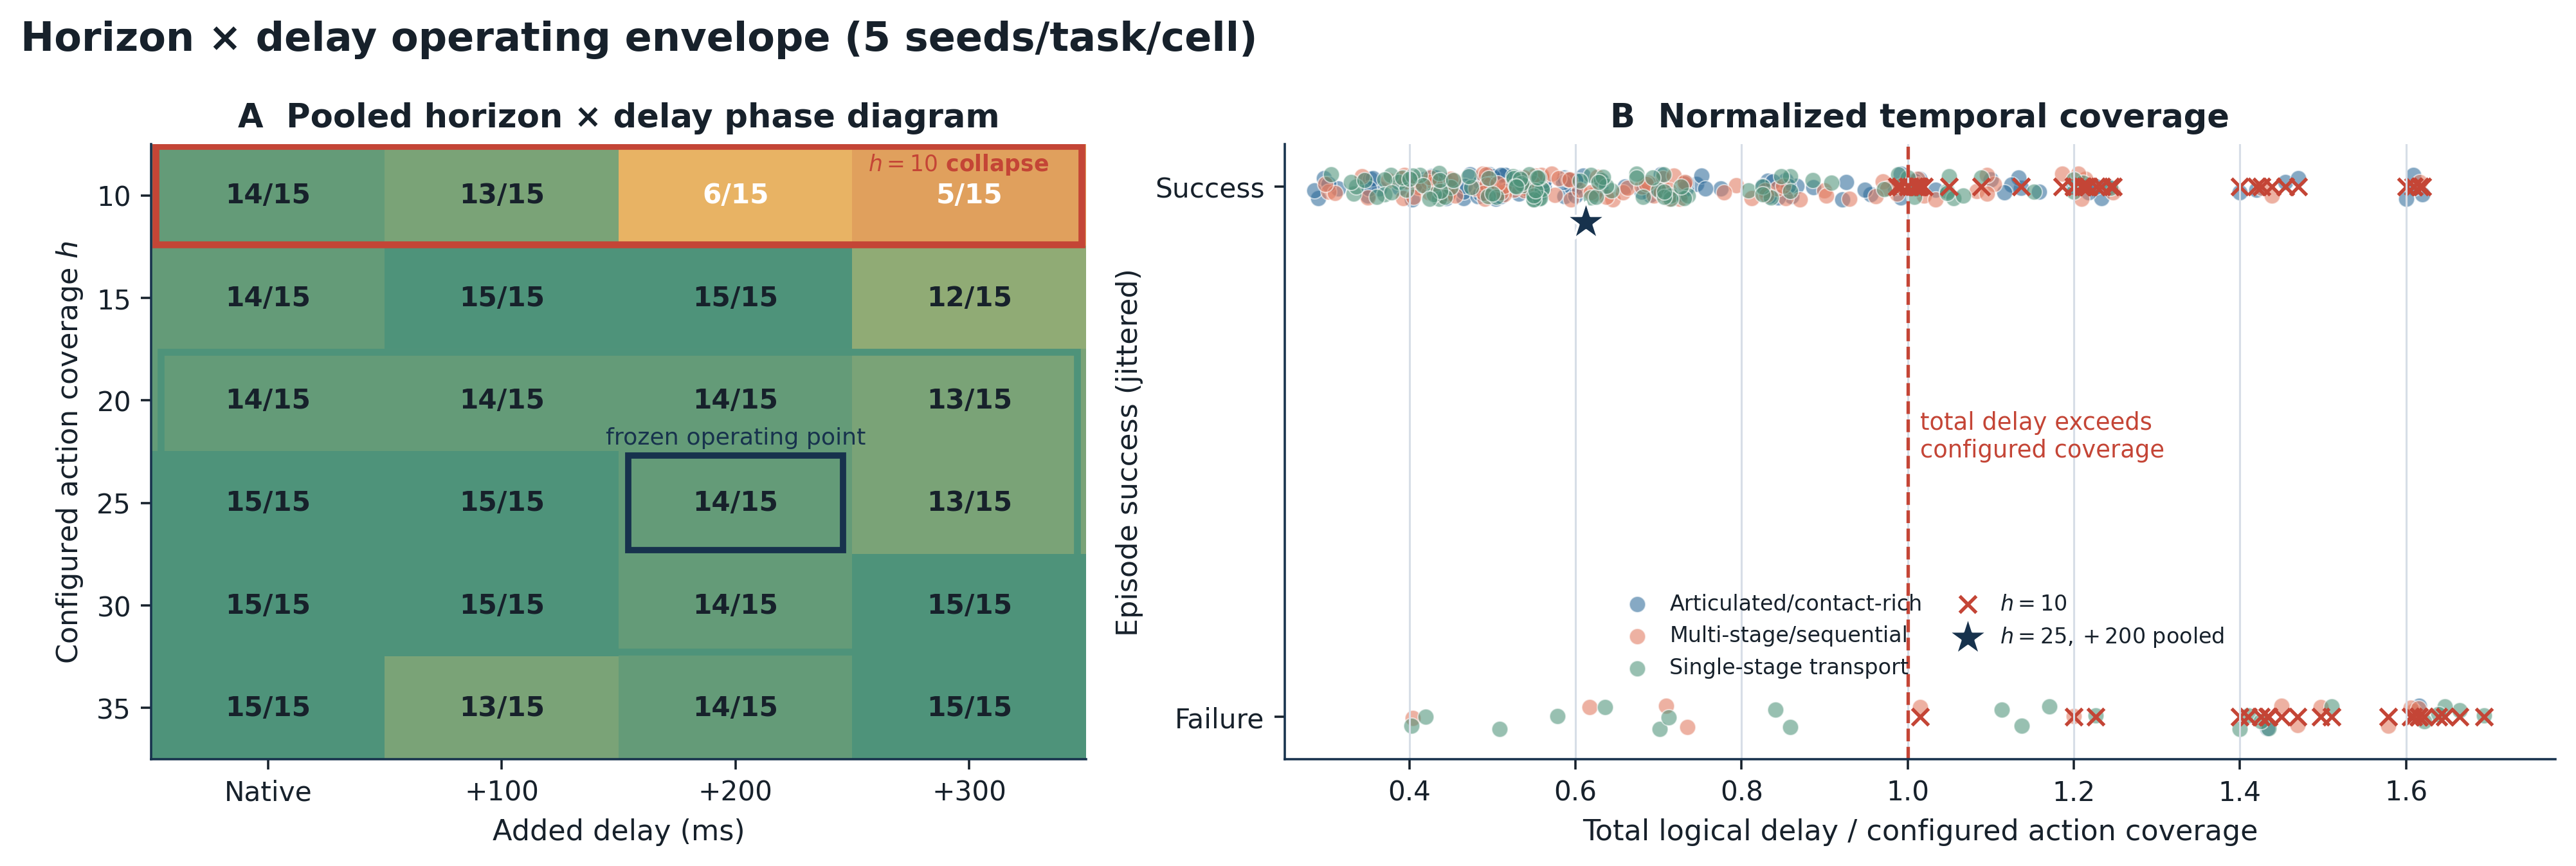
\includegraphics[width=\textwidth]{figure2_stage2_operating_envelope.png}
    \caption{Horizon--delay operating envelope under RTC. Left: pooled successes across three tasks (five seeds per task and cell). Right: episode outcomes plotted against total logical delay normalized by configured action coverage. The star marks the frozen operating point.}
    \label{fig:operating_envelope}
\end{figure}

RTC achieves substantially higher absolute success than Naive Async in this experiment. However, the main question here is the interaction with distribution shift rather than the absolute method ranking. Neither method shows evidence that the +200 ms delay becomes broadly more harmful under OOD conditions. We therefore examine whether stronger interactions are localized to individual task--perturbation combinations.

\begin{figure}[t]
    \centering
    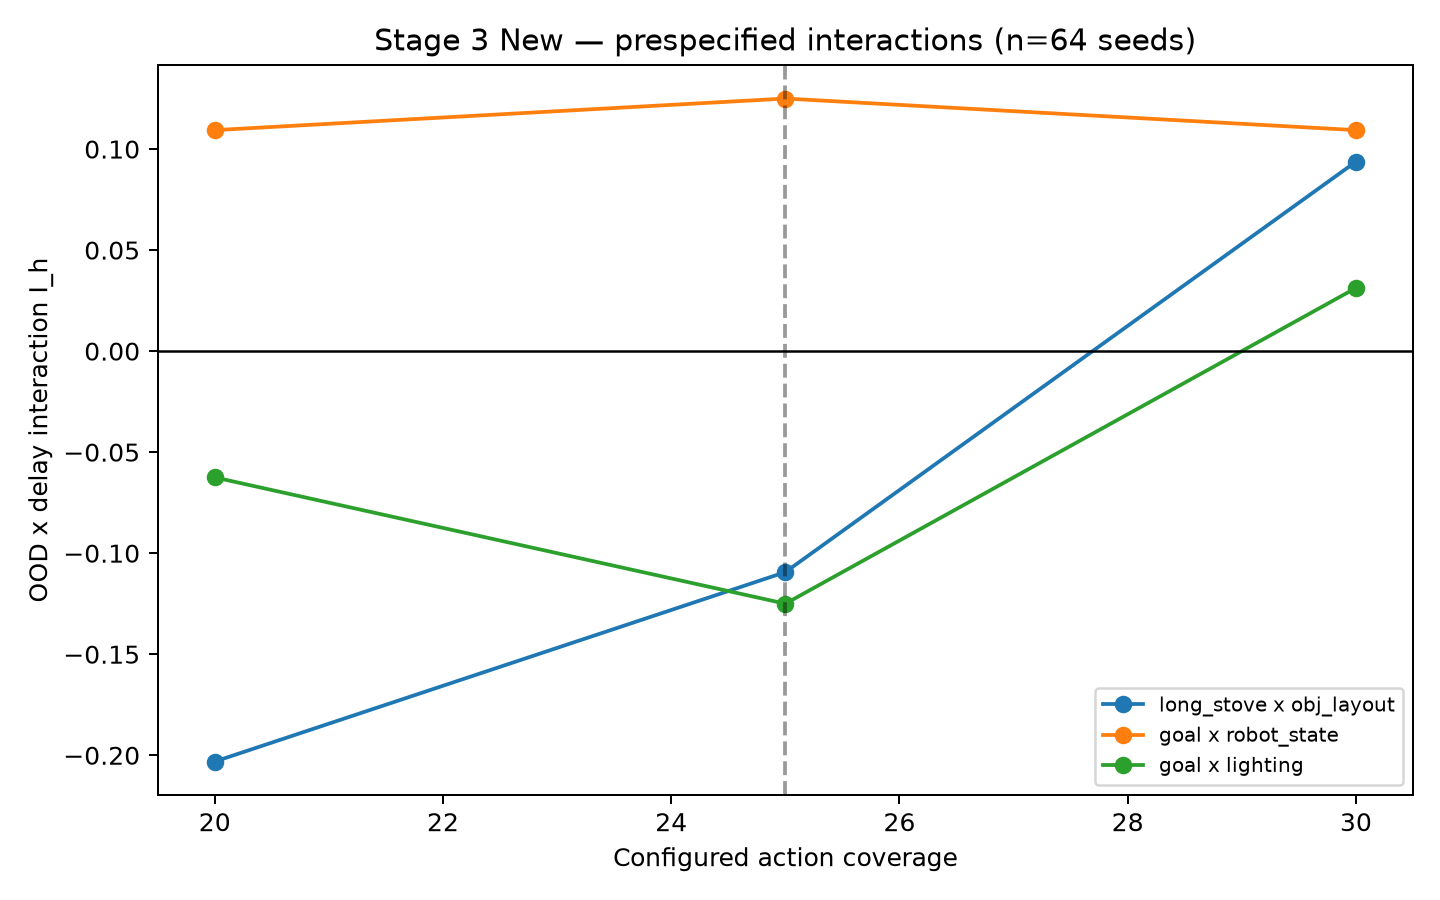
\includegraphics[width=0.82\textwidth]{figure4_stage3_stage3b_replication.png}
    \caption{Prespecified held-out OOD--delay interactions from the 64-seed replication. Lines show paired point estimates across configured action coverages; the dashed line marks the frozen $h=25$ operating point. Corresponding paired-bootstrap intervals are reported in Table~\ref{tab:stage3_confirmation}.}
    \label{fig:heldout_replication}
\end{figure}

\begin{table}[t]
\centering
\small
\caption{64-seed OOD--delay interactions for object-layout perturbations across tasks. Entries report \(I\) with paired-bootstrap 95\% intervals; negative values indicate a larger delay-induced drop under OOD.}
\label{tab:cross_task_object}
\begin{tabular}{l|ccc}
\hline
Task & \(h=20\) & \(h=25\) & \(h=30\) \\
\hline
Spatial transport & +0.016 [-0.031,+0.063] & 0.000 [-0.094,+0.078] & -0.031 [-0.125,+0.063] \\
Goal drawer & +0.109 [0.000,+0.219] & +0.109 [0.000,+0.219] & +0.078 [-0.047,+0.203] \\
Long stove + moka pot & -0.203 [-0.344,-0.047] & -0.109 [-0.266,+0.063] & +0.094 [-0.047,+0.234] \\
\hline
\end{tabular}
\end{table}

\subsection{High-Power Held-Out Replication Shows Horizon-Dependent Effects}

The 64-seed fresh-rollout replication does not support a consistently negative interaction for the long-stove/object-layout pair. Its estimates are \(I=-0.203\), \(-0.109\), and \(+0.094\) for \(h=20\), \(25\), and \(30\), respectively; only the \(h=20\) interval excludes zero. The goal-drawer/robot-initial-state candidate is positive at all three horizons, with a paired-bootstrap interval excluding zero at \(h=25\), while the lighting candidate is mixed and all of its intervals include zero. Thus the sign and magnitude of local interactions depend on both task and action coverage.

We then evaluate object-layout perturbations across three tasks. Figure~\ref{fig:heldout_replication} visualizes the prespecified candidate estimates, while Table~\ref{tab:cross_task_object} reports the 64-seed object-layout comparisons with intervals. The spatial-transport effects are near zero, the goal-drawer effects are positive, and the long-stove effects change sign with horizon. Object-layout perturbations therefore do not generally reduce delay tolerance; the interaction depends on the task and operating horizon.

\subsection{Layout and Cross-Task Generalization}

The original layout-level generalization experiments remain an exploratory eight-seed analysis. To determine whether the earlier long-stove effect was caused by a single object configuration, we evaluate three additional object-layout variants at \(h=25\). The variants produce interactions of \(-0.375\), \(+0.125\), and \(-0.125\). These estimates are mixed and should not be interpreted as a powered confirmation of a task-wide effect.

We additionally test three object-layout variants on a second multi-stage manipulation task, putting both the alphabet soup and the tomato sauce in the bucket. Here, the interactions are \(-0.375\), \(+0.250\), and \(+0.625\), with a mean interaction of \(+0.167\). This exploratory analysis provides no evidence that multi-stage or sequential tasks are generally more vulnerable to the combination of distribution shift and inference delay. Figure~\ref{fig:layout_generalization} summarizes the layout-level OOD--delay interaction estimates and paired-bootstrap confidence intervals across both tasks.

\begin{figure}[t]
    \centering
    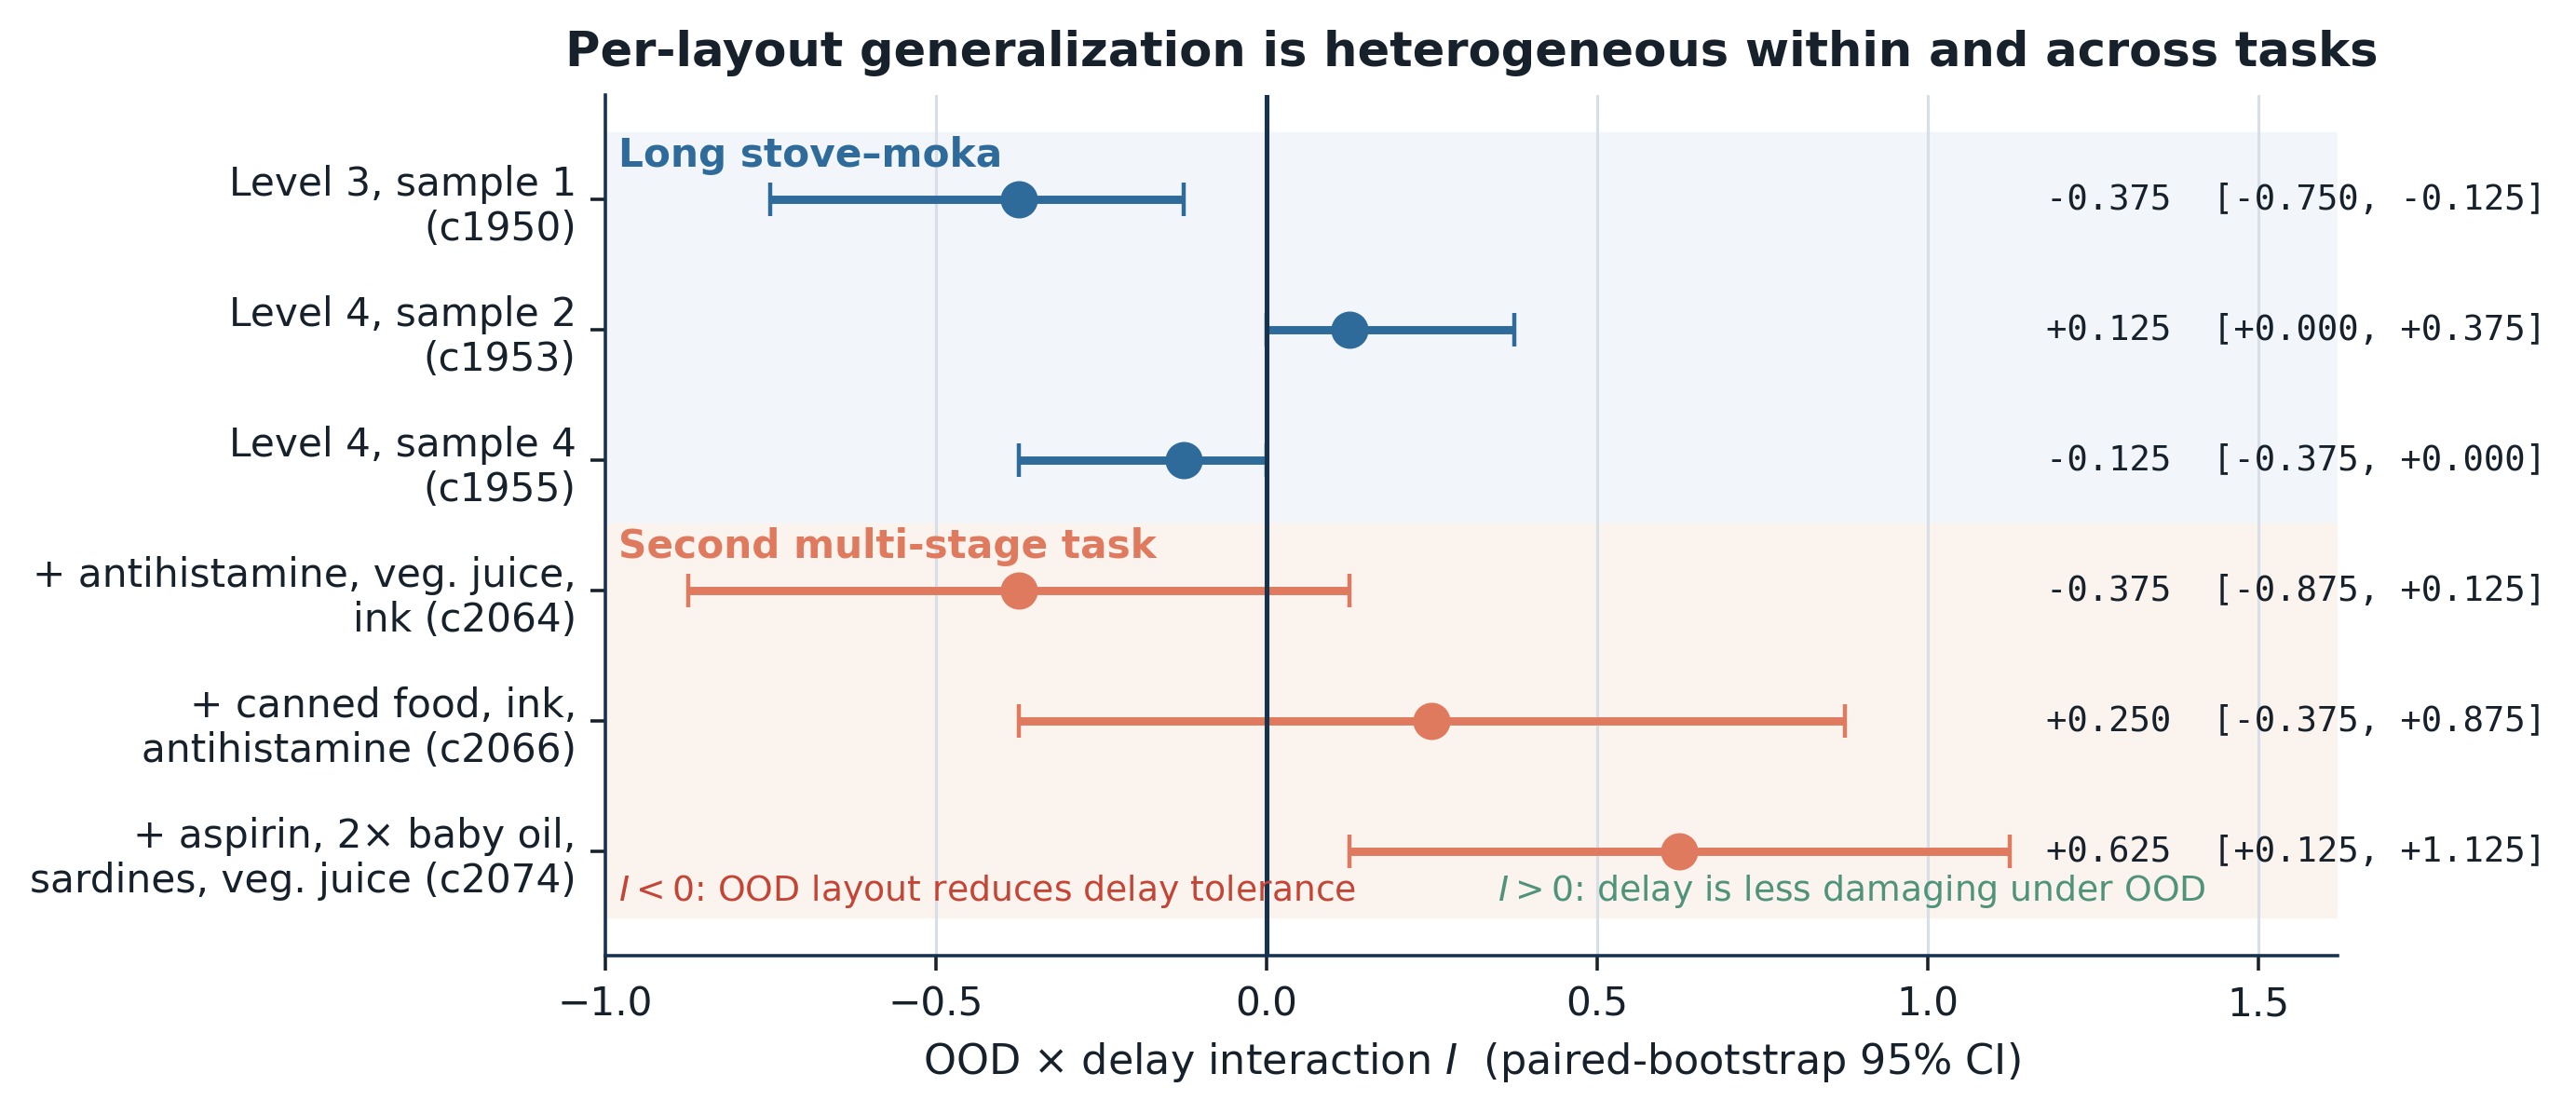
\includegraphics[width=\textwidth]{figure5_experiments_a_b_layout_generalization_compact.png}
    \caption{Layout and task--level OOD--delay interactions at \(h=25\). Points are paired estimates; bars are paired-seed bootstrap 95\% CIs. Labels include LIBERO-Plus classification IDs.}
    \label{fig:layout_generalization}
\end{figure}

\section{Conclusion}

We investigated if controlled distribution shifts amplify the effect of inference delay during asynchronous VLA execution. Across a 480-episode screen spanning three LIBERO tasks, seven LIBERO-Plus perturbation families, two execution methods, and matched Native and \(+200\,\mathrm{ms}\) conditions, the pooled OOD--delay interaction was \(I=+0.014\). A subsequent 64-seed follow-up produced 3,456 valid episodes across six candidate task--perturbation pairs and three horizons. Together, these experiments do not support the claim that OOD conditions broadly increase the delay-induced loss in task success.

Temporal action coverage produced a more consistent effect. Under RTC at \(+200\,\mathrm{ms}\), pooled success was \(6/15\) with an execution horizon of 10 actions, compared with \(14/15\) at each of \(h \in \{20,25,30\}\). The short-horizon condition also produced 1,385 queue-underrun control steps, whereas no underruns occurred at the tested \(+200\,\mathrm{ms}\) operating points for \(h \geq 20\). These results indicate that asynchronous performance can degrade sharply when total request latency approaches or exceeds the temporal coverage provided by the queued actions.

The high-power held-out experiments show that local interactions can occur, but they are task- and horizon-dependent. The long-stove/object-layout estimate changes from negative at \(h=20\) and \(25\) to positive at \(h=30\), while the goal-drawer/robot-initial-state estimate is positive and the lighting estimate is mixed. Most intervals include zero, so these results do not establish a universal heterogeneous-interaction pattern or broad OOD amplification. The separate layout-generalization experiments use eight seeds per cell and remain exploratory.

Our evaluation is limited to one \(\pi_{0.5}\) checkpoint, three simulated tasks, and benchmark-provided OOD variants whose requested initialization indices resolve to a single reset state. The rollout seeds therefore measure stochastic policy variation rather than robustness across distinct initializations. Future evaluations should expand initialization diversity, policies, tasks, and real-world settings. Asynchronous VLA benchmarks should calibrate inference delay relative to available action coverage, report queue underruns alongside task success, and test candidate OOD--delay effects across multiple tasks and scene variants.

{
\small


\begin{thebibliography}{9}

\bibitem{1}
Zhao, T. Z., Kumar, V., Levine, S., \& Finn, C. (2023).
\textit{Learning fine-grained bimanual manipulation with low-cost hardware}
[Preprint]. arXiv.
\url{https://arxiv.org/abs/2304.13705}

\bibitem{2}
Intelligence, P., Black, K., Brown, N., Darpinian, J., Dhabalia, K., Driess, D., ... \& Zhilinsky, U. (2025). $\pi_ {0.5} $: a Vision-Language-Action Model with Open-World Generalization.
arXiv preprint
\url{https://arXiv:2504.16054}

\bibitem{3}
Black, K., Galliker, M., \& Levine, S. (2026). Real-time execution of action chunking flow policies. Advances in Neural Information Processing Systems, 38, 33383-33407.

\bibitem{4}
Agouzoul, A. (2026). Understanding asynchronous inference methods for vision-language-action models. arXiv preprint
\url{https://arXiv:2605.08168}.

\bibitem{5}
Fei, S., Wang, S., Shi, J., Dai, Z., Cai, J., Qian, P., ... \& Qiu, X. (2025). Libero-plus: In-depth robustness analysis of vision-language-action models. arXiv preprint
\url{https://arXiv:2510.13626}.

\bibitem{6}
Liu, B., Zhu, Y., Gao, C., Feng, Y., Liu, Q., Zhu, Y., \& Stone, P. (2023). Libero: Benchmarking knowledge transfer for lifelong robot learning. Advances in Neural Information Processing Systems, 36, 44776-44791.

\bibitem{8}
Chi, C., Xu, Z., Feng, S., Cousineau, E., Du, Y., Burchfiel, B., ...\& Song, S. (2025). Diffusion policy: Visuomotor policy learning via action diffusion. The International Journal of Robotics Research, 44(10-11), 1684-1704.

\bibitem{9}
Black, K., Brown, N., Driess, D., Esmail, A., Equi, M., Finn, C., ... \& Zhilinsky, U. (2024). $\pi_0 $: A Vision-Language-Action Flow Model for General Robot Control. arXiv preprint
\url{https://arXiv:2410.24164}.

\bibitem{10}
Black, K., Brown, N., Darpinian, J., Dhabalia, K., Driess, D., Esmail, A., Equi, M.R., Finn, C., Fusai, N., Galliker, M.Y., Ghosh, D., Groom, L., Hausman, K., ichter, b., Jakubczak, S., Jones, T., Ke, L., LeBlanc, D., Levine, S., Li-Bell, A., Mothukuri, M., Nair, S., Pertsch, K., Ren, A.Z., Shi, L.X., Smith, L., Springenberg, J.T., Stachowicz, K., Tanner, J., Vuong, Q., Walke, H., Walling, A., Wang, H., Yu, L. \&amp; Zhilinsky, U.. (2025). $\pi_0.5$: a Vision-Language-Action Model with Open-World Generalization. <i>Proceedings of The 9th Conference on Robot Learning</i>, in <i>Proceedings of Machine Learning Research</i> 305:17-40 Available from https://proceedings.mlr.press/v305/black25a.html.

\bibitem{11}
Sendai, K., Alvarez, M., Matsushima, T., Matsuo, Y., \& Iwasawa, Y. (2025). Leave no observation behind: Real-time correction for vla action chunks. arXiv preprint
\url{https://arXiv:2509.23224}.

\bibitem{12}
Wang, H., Zhang, G., Yan, Y., Kompella, R. R., \& Liu, G. (2026). VLA Knows Its Limits: Adaptive Execution Horizons for Robot Policies. arXiv preprint
\url{https://arXiv:2602.21445}.

\bibitem{13}
Zhao, Y., Bogdanovic, M., Sohal, A., Tao, L., Darvish, K., Aspuru-Guzik, A., ... \& Garg, A. (2026). Dynamic Execution Horizon Prediction for Chunk-based Robot Policies. arXiv preprint
\url{https://arXiv:2606.11408}.

\bibitem{14}
Tang, J., Sun, Y., Zhao, Y., Yang, S., Lin, Y., Zhang, Z., ... \& Han, S. (2025). Vlash: Real-time vlas via future-state-aware asynchronous inference. arXiv preprint
\url{arXiv:2512.01031}.

\bibitem{15}
Guo, T., \& Guo, M. (2026). Action ControlNet: A Lightweight Delay-Aware Adapter for Smooth Asynchronous Control in Vision-Language-Action Models. arXiv preprint
\url{https://arXiv:2606.25985}.

\bibitem{16}
Black, K., Ren, A. Z., Equi, M., \& Levine, S. (2025). Training-time action conditioning for efficient real-time chunking. arXiv preprint \url{https://arXiv:2512.05964}.

\bibitem{17}
Jiang, H., Zou, Y., Liang, B., Liu, B., Meng, F., \& Liu, S. (2026). FutureRTC: Real-Time Robot Execution with Anticipatory-Conditioned Action Chunking. arXiv preprint

\url{https://arXiv:2607.24008}.

\bibitem{18}
Agouzoul, A. (2026). Understanding asynchronous inference methods for vision-language-action models. arXiv preprint
\url{https://arXiv:2605.08168}.

\bibitem{19}
Li, X., Hsu, K., Gu, J., Pertsch, K., Mees, O., Walke, H. R., ... \& Xiao, T. (2024). Evaluating real-world robot manipulation policies in simulation. arXiv preprint arXiv:2405.05941.

\bibitem{20}
Gao, J., Belkhale, S., Dasari, S., Balakrishna, A., Shah, D., \& Sadigh, D. (2026). A taxonomy for evaluating generalist robot manipulation policies. IEEE Robotics and Automation Letters.

\bibitem{21}
Guo, J., Wu, Z., Tu, C., Ma, Y., Kong, X., Liu, Z., ... \& Li, S. (2026, April). On robustness of vision-language-action model against multi-modal perturbations. In International Conference on Learning Representations (Vol. 2026, pp. 70248-70272).

\bibitem{22}
Li, W., Zhang, Q., Zhai, R., Lin, L., \& Wang, G. (2026). Vla models are more generalizable than you think: Revisiting physical and spatial modeling. In Proceedings of the IEEE/CVF Conference on Computer Vision and Pattern Recognition (pp. 35025-35035).

\end{thebibliography}
}


%%%%%%%%%%%%%%%%%%%%%%%%%%%%%%%%%%%%%%%%%%%%%%%%%%%%%%%%%%%%

\appendix

\section{Appendix}

\subsection{Latency Calibration}

Before the main OOD evaluation, we perform a latency calibration to select an added-delay condition that produces a measurable but non-catastrophic degradation. Table~\ref{tab:calibration} reports success over the viable task--method cells. Native performance is 87.5\%, while +200 ms reduces success to 66.7\%. We therefore use +200 ms as the primary high-delay condition in the subsequent OOD experiments.

Twenty-four Stage 0 ID-control episodes were reused in Stage 1 and lack immutable runtime-identity metadata;
we therefore retain their unverified-provenance lab

\begin{table}[h]
\centering
\small
\caption{Stage 0 latency calibration over viable ID task--method cells.}
\label{tab:calibration}
\begin{tabular}{l|c|c|c|c}
\hline
Added delay & Success & Rate & Mean request latency & p95 action age \\
\hline
Native & 21/24 & 87.5\% & 617.9 ms & 1275.0 ms \\
+100 ms & 19/24 & 79.2\% & 616.0 ms & 1457.5 ms \\
+200 ms & 16/24 & 66.7\% & 629.2 ms & 1680.5 ms \\
+300 ms & 17/24 & 70.8\% & 629.1 ms & 1872.8 ms \\
+400 ms & 17/24 & 70.8\% & 640.9 ms & 2077.1 ms \\
\hline
\end{tabular}
\end{table}

\subsection{Queue Underruns Across the Horizon Sweep}

Table~\ref{tab:full_underruns} reports the total number of queue-underrun control steps during the Stage 2 horizon sweep. Underruns increase sharply at \(h=10\), while horizons of 25 or larger avoid queue exhaustion over all tested delay conditions.

\begin{table}[h]
\centering
\small
\caption{Total queue-underrun control steps across horizons and delays.}
\label{tab:full_underruns}
\begin{tabular}{c|rrrr}
\hline
\(h\) & Native & +100 ms & +200 ms & +300 ms \\
\hline
10 & 50 & 519 & 1385 & 1765 \\
15 & 0 & 9 & 72 & 343 \\
20 & 0 & 0 & 0 & 3 \\
25 & 0 & 0 & 0 & 0 \\
30 & 0 & 0 & 0 & 0 \\
35 & 0 & 0 & 0 & 0 \\
\hline
\end{tabular}
\end{table}

\subsection{Broad Perturbation-Family Screen}

Table~\ref{tab:perturbation_full} reports the OOD--delay interaction from the initial broad screen separately for Naive Async and RTC. The broad screen contains several negative candidate effects, but the interaction is not consistently negative across perturbation families or execution methods. These cells are treated as candidate effects rather than final conclusions and are evaluated further using fresh rollouts.

\begin{table}[h]
\centering
\small
\caption{Stage 1 OOD--delay interaction \(I\) by perturbation family and execution method.}
\label{tab:perturbation_full}
\begin{tabular}{l|rr}
\hline
Perturbation & Naive Async & RTC \\
\hline
Object layout & +0.067 & -0.133 \\
Robot initial state & 0.000 & -0.067 \\
Camera viewpoint & 0.000 & +0.133 \\
Sensor noise & +0.133 & -0.067 \\
Light conditions & 0.000 & -0.067 \\
Background textures & 0.000 & +0.133 \\
Language instructions & 0.000 & +0.067 \\
\hline
\end{tabular}
\end{table}

\subsection{Fresh-Rollout Confirmatory Evaluation}

Table~\ref{tab:stage3_confirmation} reports the interaction values and paired bootstrap intervals for the 64-seed fresh-rollout replication. No prespecified candidate remains negative at all three tested horizons.

The sensor-noise and targeted object-layout rows are separately labeled post-hoc or targeted analyses and are excluded from the prespecified confirmatory claim. We compute confidence intervals from 10,000 paired bootstrap replicates by resampling the 64 rollout-seed clusters while carrying all four matched factorial cells together.

\begin{table}[h]
\centering
\small
\caption{64-seed fresh-rollout OOD--delay interactions. Values in brackets are paired bootstrap 95\% intervals from 10,000 replicates.}
\label{tab:stage3_confirmation}
\begin{tabular}{l|l|c|c}
\hline
Task & Perturbation & \(h\) & \(I\) [95\% interval] \\
\hline
Long stove & Object layout & 20 & -0.203 [-0.344,-0.047] \\
Long stove & Object layout & 25 & -0.109 [-0.266,+0.063] \\
Long stove & Object layout & 30 & +0.094 [-0.047,+0.234] \\
\hline
Goal drawer & Robot initial state & 20 & +0.109 [-0.016,+0.234] \\
Goal drawer & Robot initial state & 25 & +0.125 [+0.016,+0.234] \\
Goal drawer & Robot initial state & 30 & +0.109 [-0.016,+0.219] \\
\hline
Goal drawer & Light conditions & 20 & -0.063 [-0.188,+0.063] \\
Goal drawer & Light conditions & 25 & -0.125 [-0.281,+0.031] \\
Goal drawer & Light conditions & 30 & +0.031 [-0.109,+0.172] \\
\hline
Goal drawer & Sensor noise & 20 & +0.063 [-0.063,+0.188] \\
Goal drawer & Sensor noise & 25 & 0.000 [-0.125,+0.141] \\
Goal drawer & Sensor noise & 30 & +0.016 [-0.094,+0.141] \\
\hline
Spatial transport & Object layout & 20 & +0.016 [-0.031,+0.063] \\
Spatial transport & Object layout & 25 & 0.000 [-0.094,+0.078] \\
Spatial transport & Object layout & 30 & -0.031 [-0.125,+0.063] \\
\hline
Goal drawer & Object layout & 20 & +0.109 [0.000,+0.219] \\
Goal drawer & Object layout & 25 & +0.109 [0.000,+0.219] \\
Goal drawer & Object layout & 30 & +0.078 [-0.047,+0.203] \\
\hline
\end{tabular}
\end{table}

\subsection{Cross-Task Object-Layout Replication}

For completeness, Table~\ref{tab:cross_task_bootstrap} reports the 64-seed bootstrap intervals for the object-layout comparison across tasks. The spatial-transport effects are near zero, the goal-drawer effects are positive, and the long-stove estimates change sign with horizon.

\begin{table}[h]
\centering
\small
\caption{64-seed object-layout interaction across tasks with paired bootstrap 95\% intervals.}
\label{tab:cross_task_bootstrap}
\begin{tabular}{l|c|c}
\hline
Task & \(h\) & \(I\) [95\% interval] \\
\hline
Spatial transport & 20 & +0.016 [-0.031,+0.063] \\
Spatial transport & 25 & 0.000 [-0.094,+0.078] \\
Spatial transport & 30 & -0.031 [-0.125,+0.063] \\
\hline
Goal drawer & 20 & +0.109 [0.000,+0.219] \\
Goal drawer & 25 & +0.109 [0.000,+0.219] \\
Goal drawer & 30 & +0.078 [-0.047,+0.203] \\
\hline
Long stove & 20 & -0.203 [-0.344,-0.047] \\
Long stove & 25 & -0.109 [-0.266,+0.063] \\
Long stove & 30 & +0.094 [-0.047,+0.234] \\
\hline
\end{tabular}
\end{table}

\subsection{Layout-Level Generalization}

Tables~\ref{tab:exp_a_detail} and~\ref{tab:exp_b_detail} provide the underlying four-cell success counts for the layout-generalization experiments. All variants use \(h=25\).

\begin{table}[h]
\centering
\small
\caption{Experiment A: additional object layouts for the long-stove task.}
\label{tab:exp_a_detail}
\begin{tabular}{c|cc|cc|c}
\hline
Layout & ID Native & ID +200 & OOD Native & OOD +200 & \(I\) \\
\hline
1950 & 6/8 & 6/8 & 6/8 & 3/8 & -0.375 \\
1953 & 6/8 & 6/8 & 4/8 & 5/8 & +0.125 \\
1955 & 6/8 & 6/8 & 8/8 & 7/8 & -0.125 \\
\hline
\end{tabular}
\end{table}

\begin{table}[h]
\centering
\small
\caption{Experiment B: object-layout variants for the second multi-stage task.}
\label{tab:exp_b_detail}
\begin{tabular}{c|cc|cc|c}
\hline
Layout & ID Native & ID +200 & OOD Native & OOD +200 & \(I\) \\
\hline
2064 & 6/8 & 6/8 & 8/8 & 5/8 & -0.375 \\
2066 & 6/8 & 6/8 & 5/8 & 7/8 & +0.250 \\
2074 & 6/8 & 6/8 & 0/8 & 5/8 & +0.625 \\
\hline
\end{tabular}
\end{table}

\subsection{Initialization Audit}

We additionally audit whether the rollout seeds correspond to distinct environment initializations. For the tested OOD variants, requested initialization indices 0--7 resolve to the same environment initialization and state fingerprint. The rollout seeds should therefore be interpreted as repeated stochastic policy rollouts from a fixed OOD reset state, rather than as independent environment initializations. This limitation does not invalidate the paired rollout comparisons above, but it restricts the extent to which the results establish robustness across initialization diversity.

\subsection{Assets and Licenses}

The paper utilizes the following assets: LIBERO codebase under the MIT License,  datasets under the CC BY 4.0 License. LIBERO-Plus: perturbation assets released under the MIT License via the hugging face dataset (Sylvest/LIBERO-plus). The $\pi_{0.5}$ checkpoint used is distributed under the Gemma license.

\section*{NeurIPS Paper Checklist}


\begin{enumerate}

\item {\bf Claims}
    \item[] Question: Do the main claims made in the abstract and introduction accurately reflect the paper's contributions and scope?
    \item[] Answer: \answerYes{}
    \item[] Justification:  The abstract and introduction state the empirical scope of the paper and distinguish the pooled null OOD–delay result from the localized held-out estimates. The limitations of the evaluation, including initialization diversity, are discussed in the Conclusion and Appendix A.7.
    \item[] Guidelines:
    \begin{itemize}
        \item The answer \answerNA{} means that the abstract and introduction do not include the claims made in the paper.
        \item The abstract and/or introduction should clearly state the claims made, including the contributions made in the paper and important assumptions and limitations. A \answerNo{} or \answerNA{} answer to this question will not be perceived well by the reviewers.
        \item The claims made should match theoretical and experimental results, and reflect how much the results can be expected to generalize to other settings.
        \item It is fine to include aspirational goals as motivation as long as it is clear that these goals are not attained by the paper.
    \end{itemize}

\item {\bf Limitations}
    \item[] Question: Does the paper discuss the limitations of the work performed by the authors?
    \item[] Answer: \answerYes{} % Replace by \answerYes{}, \answerNo{}, or \answerNA{}.
    \item[] Justification: The conclusion lists the limitations of the current approach and the next steps for this work. Appendix A.7 discloses that rollout seeds should be interpreted as repeated stochastic policy rollouts from a fixed OOD reset state, rather than as independent environment initialization and that it does not invalidate the paired rollout comparisons, but it restricts the extent to which the results establish robustness across initialization diversity.
    \item[] Guidelines:
    \begin{itemize}
        \item The answer \answerNA{} means that the paper has no limitation while the answer \answerNo{} means that the paper has limitations, but those are not discussed in the paper.
        \item The authors are encouraged to create a separate ``Limitations'' section in their paper.
        \item The paper should point out any strong assumptions and how robust the results are to violations of these assumptions (e.g., independence assumptions, noiseless settings, model well-specification, asymptotic approximations only holding locally). The authors should reflect on how these assumptions might be violated in practice and what the implications would be.
        \item The authors should reflect on the scope of the claims made, e.g., if the approach was only tested on a few datasets or with a few runs. In general, empirical results often depend on implicit assumptions, which should be articulated.
        \item The authors should reflect on the factors that influence the performance of the approach. For example, a facial recognition algorithm may perform poorly when image resolution is low or images are taken in low lighting. Or a speech-to-text system might not be used reliably to provide closed captions for online lectures because it fails to handle technical jargon.
        \item The authors should discuss the computational efficiency of the proposed algorithms and how they scale with dataset size.
        \item If applicable, the authors should discuss possible limitations of their approach to address problems of privacy and fairness.
        \item While the authors might fear that complete honesty about limitations might be used by reviewers as grounds for rejection, a worse outcome might be that reviewers discover limitations that aren't acknowledged in the paper. The authors should use their best judgment and recognize that individual actions in favor of transparency play an important role in developing norms that preserve the integrity of the community. Reviewers will be specifically instructed to not penalize honesty concerning limitations.
    \end{itemize}
    % \item[] Guidelines:
    % \begin{itemize}
    %     \item The answer \answerNA{} means that the paper has no limitation while the answer \answerNo{} means that the paper has limitations, but those are not discussed in the paper.
    %     \item The authors are encouraged to create a separate ``Limitations'' section in their paper.
    %     \item The paper should point out any strong assumptions and how robust the results are to violations of these assumptions (e.g., independence assumptions, noiseless settings, model well-specification, asymptotic approximations only holding locally). The authors should reflect on how these assumptions might be violated in practice and what the implications would be.
    %     \item The authors should reflect on the scope of the claims made, e.g., if the approach was only tested on a few datasets or with a few runs. In general, empirical results often depend on implicit assumptions, which should be articulated.
    %     \item The authors should reflect on the factors that influence the performance of the approach. For example, a facial recognition algorithm may perform poorly when image resolution is low or images are taken in low lighting. Or a speech-to-text system might not be used reliably to provide closed captions for online lectures because it fails to handle technical jargon.
    %     \item The authors should discuss the computational efficiency of the proposed algorithms and how they scale with dataset size.
    %     \item If applicable, the authors should discuss possible limitations of their approach to address problems of privacy and fairness.
    %     \item While the authors might fear that complete honesty about limitations might be used by reviewers as grounds for rejection, a worse outcome might be that reviewers discover limitations that aren't acknowledged in the paper. The authors should use their best judgment and recognize that individual actions in favor of transparency play an important role in developing norms that preserve the integrity of the community. Reviewers will be specifically instructed to not penalize honesty concerning limitations.
    % \end{itemize}

\item {\bf Theory assumptions and proofs}
    \item[] Question: For each theoretical result, does the paper provide the full set of assumptions and a complete (and correct) proof?
    \item[] Answer: \answerNA{} % Replace by \answerYes{}, \answerNo{}, or \answerNA{}.
    \item[] Justification: The paper does not introduce any theoretical results or proofs.
    \item[] Guidelines:
    \begin{itemize}
        \item The answer \answerNA{} means that the paper does not include theoretical results.
        \item All the theorems, formulas, and proofs in the paper should be numbered and cross-referenced.
        \item All assumptions should be clearly stated or referenced in the statement of any theorems.
        \item The proofs can either appear in the main paper or the supplemental material, but if they appear in the supplemental material, the authors are encouraged to provide a short proof sketch to provide intuition.
        \item Inversely, any informal proof provided in the core of the paper should be complemented by formal proofs provided in appendix or supplemental material.
        \item Theorems and Lemmas that the proof relies upon should be properly referenced.
    \end{itemize}

    \item {\bf Experimental result reproducibility}
    \item[] Question: Does the paper fully disclose all the information needed to reproduce the main experimental results of the paper to the extent that it affects the main claims and/or conclusions of the paper (regardless of whether the code and data are provided or not)?
    \item[] Answer: \answerYes{}{}
    \item[] Justification: The paper specifies the policy, execution strategies, delay construction, task and perturbation setup, horizons, seed counts, and evaluation hardware. The anonymized code and accompanying documentation provide the remaining implementation and verification details needed to reproduce the benchmark.
    \item[] Guidelines:
    \begin{itemize}
        \item The answer \answerNA{} means that the paper does not include experiments.
        \item If the paper includes experiments, a \answerNo{} answer to this question will not be perceived well by the reviewers: Making the paper reproducible is important, regardless of whether the code and data are provided or not.
        \item If the contribution is a dataset and\slash or model, the authors should describe the steps taken to make their results reproducible or verifiable.
        \item Depending on the contribution, reproducibility can be accomplished in various ways. For example, if the contribution is a novel architecture, describing the architecture fully might suffice, or if the contribution is a specific model and empirical evaluation, it may be necessary to either make it possible for others to replicate the model with the same dataset, or provide access to the model. In general. releasing code and data is often one good way to accomplish this, but reproducibility can also be provided via detailed instructions for how to replicate the results, access to a hosted model (e.g., in the case of a large language model), releasing of a model checkpoint, or other means that are appropriate to the research performed.
        \item While NeurIPS does not require releasing code, the conference does require all submissions to provide some reasonable avenue for reproducibility, which may depend on the nature of the contribution. For example
        \begin{enumerate}
            \item If the contribution is primarily a new algorithm, the paper should make it clear how to reproduce that algorithm.
            \item If the contribution is primarily a new model architecture, the paper should describe the architecture clearly and fully.
            \item If the contribution is a new model (e.g., a large language model), then there should either be a way to access this model for reproducing the results or a way to reproduce the model (e.g., with an open-source dataset or instructions for how to construct the dataset).
            \item We recognize that reproducibility may be tricky in some cases, in which case authors are welcome to describe the particular way they provide for reproducibility. In the case of closed-source models, it may be that access to the model is limited in some way (e.g., to registered users), but it should be possible for other researchers to have some path to reproducing or verifying the results.
        \end{enumerate}
    \end{itemize}


\item {\bf Open access to data and code}
    \item[] Question: Does the paper provide open access to the data and code, with sufficient instructions to faithfully reproduce the main experimental results, as described in supplemental material?
    \item[] Answer: \answerYes{}
    \item[] Justification: The submission provides anonymized code with a clear \texttt{README.md} containing the environment
  setup and commands required to reproduce the main experimental results. It also includes verification notebooks that confirm the
  correct components and configurations are being executed.
    \item[] Guidelines:
    \begin{itemize}
        \item The answer \answerNA{} means that paper does not include experiments requiring code.
        \item Please see the NeurIPS code and data submission guidelines (\url{https://neurips.cc/public/guides/CodeSubmissionPolicy}) for more details.
        \item While we encourage the release of code and data, we understand that this might not be possible, so \answerNo{} is an acceptable answer. Papers cannot be rejected simply for not including code, unless this is central to the contribution (e.g., for a new open-source benchmark).
        \item The instructions should contain the exact command and environment needed to run to reproduce the results. See the NeurIPS code and data submission guidelines (\url{https://neurips.cc/public/guides/CodeSubmissionPolicy}) for more details.
        \item The authors should provide instructions on data access and preparation, including how to access the raw data, preprocessed data, intermediate data, and generated data, etc.
        \item The authors should provide scripts to reproduce all experimental results for the new proposed method and baselines. If only a subset of experiments are reproducible, they should state which ones are omitted from the script and why.
        \item At submission time, to preserve anonymity, the authors should release anonymized versions (if applicable).
        \item Providing as much information as possible in supplemental material (appended to the paper) is recommended, but including URLs to data and code is permitted.
    \end{itemize}


\item {\bf Experimental setting/details}
    \item[] Question: Does the paper specify all the training and test details (e.g., data splits, hyperparameters, how they were chosen, type of optimizer) necessary to understand the results?
    \item[] Answer: \answerYes{}
    \item[] Justification: Sections 3–4 specify the fixed policy checkpoint, execution strategies, delay construction, task and perturbation design, horizons, seed counts, and evaluation hardware. No models are trained as part of this work.
    \item[] Guidelines:
    \begin{itemize}
        \item The answer \answerNA{} means that the paper does not include experiments.
        \item The experimental setting should be presented in the core of the paper to a level of detail that is necessary to appreciate the results and make sense of them.
        \item The full details can be provided either with the code, in appendix, or as supplemental material.
    \end{itemize}

\item {\bf Experiment statistical significance}
    \item[] Question: Does the paper report error bars suitably and correctly defined or other appropriate information about the statistical significance of the experiments?
    \item[] Answer: \answerYes{}
    \item[] Justification: Figures 3–4 and Tables 6–7 report paired-bootstrap 95\% confidence intervals. Appendix A.4 describes the paired seed-cluster bootstrap procedure used for the fresh-rollout evaluation.
    \item[] Guidelines:
    \begin{itemize}
        \item The answer \answerNA{} means that the paper does not include experiments.
        \item The authors should answer \answerYes{} if the results are accompanied by error bars, confidence intervals, or statistical significance tests, at least for the experiments that support the main claims of the paper.
        \item The factors of variability that the error bars are capturing should be clearly stated (for example, train/test split, initialization, random drawing of some parameter, or overall run with given experimental conditions).
        \item The method for calculating the error bars should be explained (closed form formula, call to a library function, bootstrap, etc.)
        \item The assumptions made should be given (e.g., Normally distributed errors).
        \item It should be clear whether the error bar is the standard deviation or the standard error of the mean.
        \item It is OK to report 1-sigma error bars, but one should state it. The authors should preferably report a 2-sigma error bar than state that they have a 96\% CI, if the hypothesis of Normality of errors is not verified.
        \item For asymmetric distributions, the authors should be careful not to show in tables or figures symmetric error bars that would yield results that are out of range (e.g., negative error rates).
        \item If error bars are reported in tables or plots, the authors should explain in the text how they were calculated and reference the corresponding figures or tables in the text.
    \end{itemize}

\item {\bf Experiments compute resources}
    \item[] Question: For each experiment, does the paper provide sufficient information on the computer resources (type of compute workers, memory, time of execution) needed to reproduce the experiments?
    \item[] Answer: \answerNo{}
    \item[] Justification: Section 4.1 calls out the usage of A100 40GB HW and single GPU execution protocol, but per-experiment runtime and total project compute are not yet reported.
    \item[] Guidelines:
    \begin{itemize}
        \item The answer \answerNA{} means that the paper does not include experiments.
        \item The paper should indicate the type of compute workers CPU or GPU, internal cluster, or cloud provider, including relevant memory and storage.
        \item The paper should provide the amount of compute required for each of the individual experimental runs as well as estimate the total compute.
        \item The paper should disclose whether the full research project required more compute than the experiments reported in the paper (e.g., preliminary or failed experiments that didn't make it into the paper).
    \end{itemize}

\item {\bf Code of ethics}
    \item[] Question: Does the research conducted in the paper conform, in every respect, with the NeurIPS Code of Ethics \url{https://neurips.cc/public/EthicsGuidelines}?
    \item[] Answer: \answerYes{}
    \item[] Justification: Paper involves simulation benchmarking and does not involve human subject data.
    \item[] Guidelines:
    \begin{itemize}
        \item The answer \answerNA{} means that the authors have not reviewed the NeurIPS Code of Ethics.
        \item If the authors answer \answerNo, they should explain the special circumstances that require a deviation from the Code of Ethics.
        \item The authors should make sure to preserve anonymity (e.g., if there is a special consideration due to laws or regulations in their jurisdiction).
    \end{itemize}


\item {\bf Broader impacts}
    \item[] Question: Does the paper discuss both potential positive societal impacts and negative societal impacts of the work performed?
    \item[] Answer: \answerNA{}% Replace by \answerYes{}, \answerNo{}, or \answerNA{}.
    \item[] Justification: This work evaluates simulated robot-control policies and does not introduce a deployed system or application with a direct societal impact requiring separate analysis.
    \item[] Guidelines:
    \begin{itemize}
        \item The answer \answerNA{} means that there is no societal impact of the work performed.
        \item If the authors answer \answerNA{} or \answerNo, they should explain why their work has no societal impact or why the paper does not address societal impact.
        \item Examples of negative societal impacts include potential malicious or unintended uses (e.g., disinformation, generating fake profiles, surveillance), fairness considerations (e.g., deployment of technologies that could make decisions that unfairly impact specific groups), privacy considerations, and security considerations.
        \item The conference expects that many papers will be foundational research and not tied to particular applications, let alone deployments. However, if there is a direct path to any negative applications, the authors should point it out. For example, it is legitimate to point out that an improvement in the quality of generative models could be used to generate Deepfakes for disinformation. On the other hand, it is not needed to point out that a generic algorithm for optimizing neural networks could enable people to train models that generate Deepfakes faster.
        \item The authors should consider possible harms that could arise when the technology is being used as intended and functioning correctly, harms that could arise when the technology is being used as intended but gives incorrect results, and harms following from (intentional or unintentional) misuse of the technology.
        \item If there are negative societal impacts, the authors could also discuss possible mitigation strategies (e.g., gated release of models, providing defenses in addition to attacks, mechanisms for monitoring misuse, mechanisms to monitor how a system learns from feedback over time, improving the efficiency and accessibility of ML).
    \end{itemize}


\item {\bf Safeguards}
    \item[] Question: Does the paper describe safeguards that have been put in place for responsible release of data or models that have a high risk for misuse (e.g., pre-trained language models, image generators, or scraped datasets)?
    \item[] Answer: \answerNA{} % Replace by \answerYes{}, \answerNo{}, or \answerNA{}.
    \item[] Justification: Paper on simulation benchmarking and retrospection rather than a high-risk release
    \item[] Guidelines:
    \begin{itemize}
        \item The answer \answerNA{} means that the paper poses no such risks.
        \item Released models that have a high risk for misuse or dual-use should be released with necessary safeguards to allow for controlled use of the model, for example by requiring that users adhere to usage guidelines or restrictions to access the model or implementing safety filters.
        \item Datasets that have been scraped from the Internet could pose safety risks. The authors should describe how they avoided releasing unsafe images.
        \item We recognize that providing effective safeguards is challenging, and many papers do not require this, but we encourage authors to take this into account and make a best faith effort.
    \end{itemize}

\item {\bf Licenses for existing assets}
    \item[] Question: Are the creators or original owners of assets (e.g., code, data, models), used in the paper, properly credited and are the license and terms of use explicitly mentioned and properly respected?
    \item[] Answer: \answerYes{} % Replace by \answerYes{}, \answerNo{}, or \answerNA{}.
    \item[] Justification: The paper uses LIBERO (MIT License for code and CC BY 4.0 for datasets), LIBERO-Plus (MIT License), and the $\pi_{0.5}$ checkpoint (Gemma License). These assets and licenses are documented in Appendix A.8 and the corresponding works are cited.
    \item[] Guidelines:
    \begin{itemize}
        \item The answer \answerNA{} means that the paper does not use existing assets.
        \item The authors should cite the original paper that produced the code package or dataset.
        \item The authors should state which version of the asset is used and, if possible, include a URL.
        \item The name of the license (e.g., CC-BY 4.0) should be included for each asset.
        \item For scraped data from a particular source (e.g., website), the copyright and terms of service of that source should be provided.
        \item If assets are released, the license, copyright information, and terms of use in the package should be provided. For popular datasets, \url{paperswithcode.com/datasets} has curated licenses for some datasets. Their licensing guide can help determine the license of a dataset.
        \item For existing datasets that are re-packaged, both the original license and the license of the derived asset (if it has changed) should be provided.
        \item If this information is not available online, the authors are encouraged to reach out to the asset's creators.
    \end{itemize}

\item {\bf New assets}
    \item[] Question: Are new assets introduced in the paper well documented and is the documentation provided alongside the assets?
    \item[] Answer: \answerYes{} % Replace by \answerYes{}, \answerNo{}, or \answerNA{}.
    \item[] Justification: We release the benchmark implementation used in this work through the anonymized repository linked in the paper. The repository includes setup instructions, experiment commands, and verification utilities.
    \item[] Guidelines:
    \begin{itemize}
        \item The answer \answerNA{} means that the paper does not release new assets.
        \item Researchers should communicate the details of the dataset\slash code\slash model as part of their submissions via structured templates. This includes details about training, license, limitations, etc.
        \item The paper should discuss whether and how consent was obtained from people whose asset is used.
        \item At submission time, remember to anonymize your assets (if applicable). You can either create an anonymized URL or include an anonymized zip file.
    \end{itemize}


\item {\bf Crowdsourcing and research with human subjects}
    \item[] Question: For crowdsourcing experiments and research with human subjects, does the paper include the full text of instructions given to participants and screenshots, if applicable, as well as details about compensation (if any)?
    \item[] Answer: \answerNA % Replace by \answerYes{}, \answerNo{}, or \answerNA{}.
    \item[] Justification: No crowd sourcing experiments were conducted during this work.
    \item[] Guidelines:
    \begin{itemize}
        \item The answer \answerNA{} means that the paper does not involve crowdsourcing nor research with human subjects.
        \item Including this information in the supplemental material is fine, but if the main contribution of the paper involves human subjects, then as much detail as possible should be included in the main paper.
        \item According to the NeurIPS Code of Ethics, workers involved in data collection, curation, or other labor should be paid at least the minimum wage in the country of the data collector.
    \end{itemize}

\item {\bf Institutional review board (IRB) approvals or equivalent for research with human subjects}
    \item[] Question: Does the paper describe potential risks incurred by study participants, whether such risks were disclosed to the subjects, and whether Institutional Review Board (IRB) approvals (or an equivalent approval/review based on the requirements of your country or institution) were obtained?
    \item[] Answer: \answerNA{} % Replace by \answerYes{}, \answerNo{}, or \answerNA{}.
    \item[] Justification: The paper does not involve crowdsourcing nor research with human subjects.
    \item[] Guidelines:
    \begin{itemize}
        \item The answer \answerNA{} means that the paper does not involve crowdsourcing nor research with human subjects.
        \item Depending on the country in which research is conducted, IRB approval (or equivalent) may be required for any human subjects research. If you obtained IRB approval, you should clearly state this in the paper.
        \item We recognize that the procedures for this may vary significantly between institutions and locations, and we expect authors to adhere to the NeurIPS Code of Ethics and the guidelines for their institution.
        \item For initial submissions, do not include any information that would break anonymity (if applicable), such as the institution conducting the review.
    \end{itemize}

\item {\bf Declaration of LLM usage}
    \item[] Question: Does the paper describe the usage of LLMs if it is an important, original, or non-standard component of the core methods in this research? Note that if the LLM is used only for writing, editing, or formatting purposes and does \emph{not} impact the core methodology, scientific rigor, or originality of the research, declaration is not required.
    %this research?
    \item[] Answer: \answerYes{} % Replace by \answerYes{}, \answerNo{}, or \answerNA{}.
    \item[] Justification: LLMs were used for editing assistance and for brainstorming possible experimental configurations and design choices. All experimental protocols, implementation decisions, analyses, and conclusions were independently reviewed and validated by the authors, who take full responsibility for the reported results.
    \item[] Guidelines:
    \begin{itemize}
        \item The answer \answerNA{} means that the core method development in this research does not involve LLMs as any important, original, or non-standard components.
        \item Please refer to our LLM policy in the NeurIPS handbook for what should or should not be described.
    \end{itemize}

\end{enumerate}



\end{document}
